\documentclass[10pt]{article}
\usepackage[letterpaper,margin=0.8in]{geometry}
\usepackage{amsmath,amssymb,booktabs,graphicx,array}
\usepackage[T1]{fontenc}
\usepackage{lmodern}
\usepackage[hidelinks]{hyperref}
\usepackage{xurl}
\setlength{\parindent}{0pt}
\setlength{\parskip}{4pt}
\newcommand{\StrictIntegerCount}{32}
\newcommand{\StrictIntegerPct}{0.6529}
\newcommand{\StrictEffectiveCount}{4}
\newcommand{\StrictLabels}{29}
\newcommand{\StrictLabelsPct}{0.6473}
\newcommand{\InclusiveLabels}{30}
\newcommand{\InclusiveIntegerCount}{0}

\makeatletter
\renewcommand{\maketitle}{\begin{center}{\Large\bfseries\@title\par}\vspace{5pt}\@author\qquad\@date\end{center}}
\makeatother
\setlength{\intextsep}{7pt}
\setlength{\abovecaptionskip}{5pt}
\title{Cutoff Sensitivity of Strict Splitting Counts\\
\large An Exact Extension to 5000 on the Fixed Curve Cohort}
\author{Anonymous}
\date{30 October 2026}
\begin{document}
\maketitle
\begin{abstract}
We extend the previously reported strict Frobenius-discriminant splitting-count
comparison to every integer cutoff from 100 through 5000, retaining all 21
curve rows and enumerating all 4480 original stream-count-preserving label
assignments. The observed within-field separation occurs only at
$691\le L\le718$ and $769\le L\le772$: \StrictIntegerCount{} of 4901 integer
cutoffs (\StrictIntegerPct\%). No cutoff above 772 separates the paired
publications and named unpublished candidates. A separate native implementation
reconstructs all five output files; three deliberate corruptions are refused.
This is retrospective exact reanalysis, with no new curves or point counts.
It establishes cutoff sensitivity in this cohort, not a historical selection
rule, unusualness against random curves, or an ECDLP advantage.
\end{abstract}

\section{Question and fixed method}
The original degree-691 observation was reported before this work~\cite{asanso,replication}.
For each inherited cofactor-one curve, with certified full order $n$, set
\[
 t=p+1-n,\qquad \Delta=t^2-4p,\qquad
 S_L=\#\{\text{odd primes }\ell\le L:(\Delta/\ell)=+1\}.
\]
We retain ramified characters separately as $R_L$ and report $S_L+R_L$ only as
a sensitivity analysis. Prime 2 is exceptional and has no computed Legendre
character. The count is a property of $p,n$; changing the base point does not
change it. Background on Elkies/Atkin characters does not provide a finite
conditional random-curve model for these inputs~\cite{ss}.

For each of the four fields with both labels, define
$m_L=\min_{\rm unpublished}S_L-\max_{\rm published}S_L$.
The joint rule succeeds exactly when all four margins are positive. The
384-/521-bit publications remain in the data without invented same-field
comparison margins. Every integer cutoff is retained; 645 effective positions
represent the requested range.

\begin{figure}[!ht]
\centering
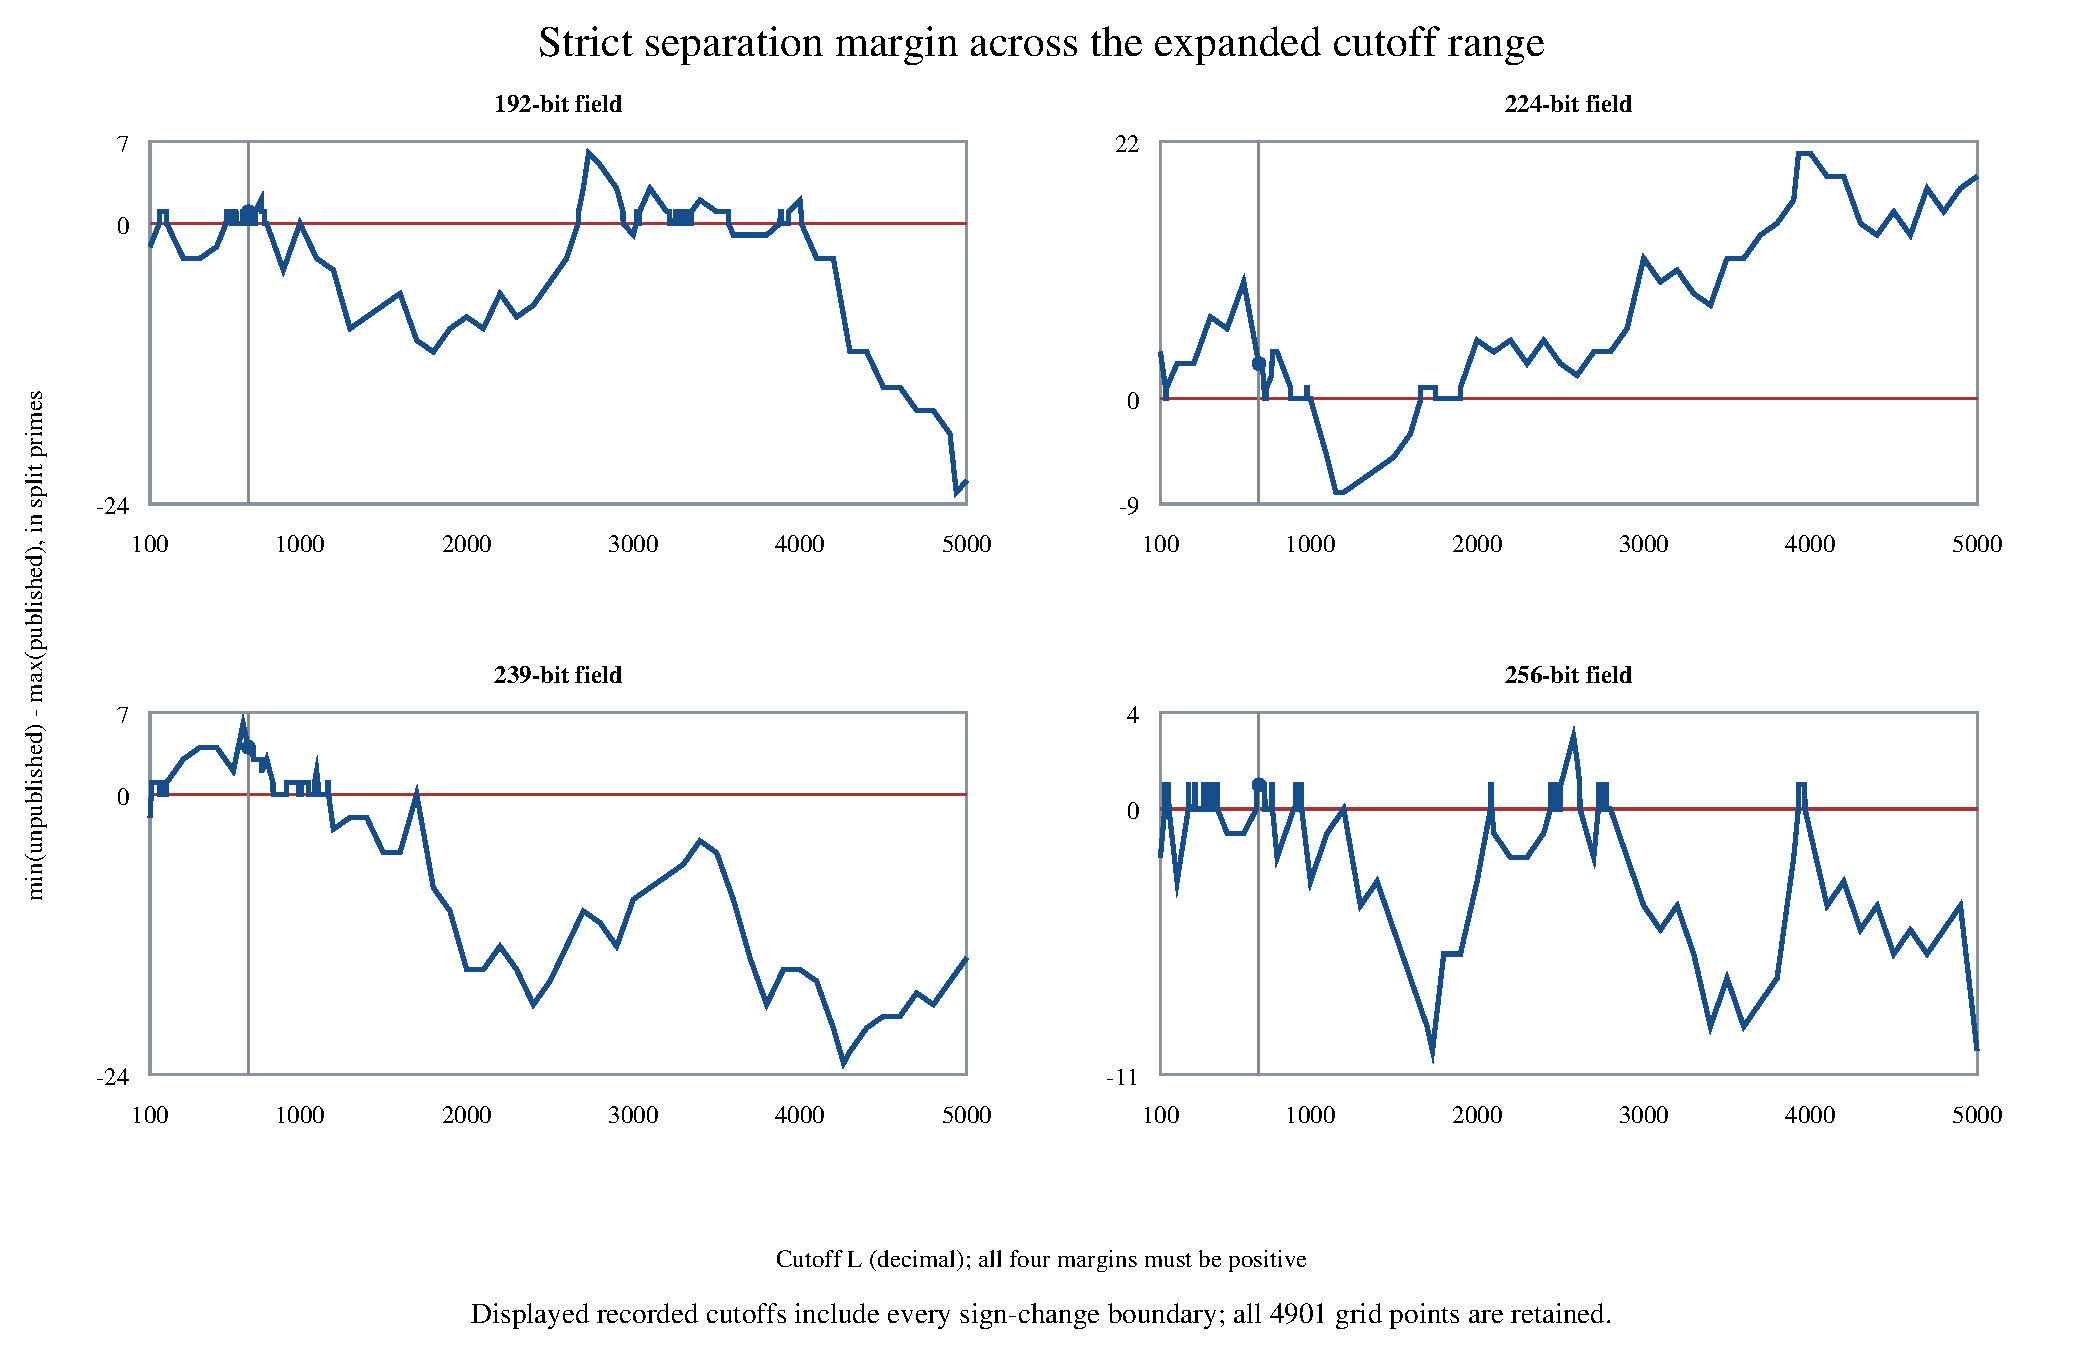
\includegraphics[width=0.92\linewidth]{figures/cutoff-margins.pdf}
\caption{Recorded strict margins in the fixed cohort. The horizontal line is
zero; the vertical marker is 691. Display points include a 100-step grid,
691, all sign-change boundaries, extrema and joint-success boundaries.
Lines guide the eye; all 4901 integer positions are retained in the raw data.
These are exact finite counts, so sampling-error bars are inapplicable.}
\label{fig:margins}
\end{figure}
\clearpage

\section{Full-range results}
The only strict success intervals are $[691,718]$ and $[769,772]$, inclusive.
They contain 32 integer cutoffs and four effective prime cutoffs:
691, 701, 709 and 769. Thus the ordering holds at \StrictIntegerPct\%{} of
the integer grid and at 0.6202\% of effective positions. It fails at every
cutoff from 773 through 5000. Including ramified primes yields
\emph{zero} joint-success cutoffs in the requested range.

\begin{table}[!ht]
\centering
\begin{tabular}{rrrrr}
\toprule
Field bits & Positive cutoffs & Percent & $m_{691}$ & $m_{5000}$ \\
\midrule
192 & 1018 & 20.7713 & 1 & -22 \\
224 & 3957 & 80.7386 & 3 & 19 \\
239 & 862 & 17.5882 & 4 & -14 \\
256 & 374 & 7.6311 & 1 & -10 \\
\bottomrule
\end{tabular}

\caption{Within-field strict ordering across all 4901 integer cutoffs.
A positive margin means every paired publication has a smaller count than
every named unpublished candidate in that field. The percentages describe this
grid, not a sampling probability or statistical comparison between fields.}
\label{tab:fields}
\end{table}

P-224 is the more persistent case within this cohort. At 5000 its publication
has strict count 299, compared with 318, 342 and 325 for its three controls.
The other three paired fields have negative margins at 5000. Their
publication/control ordering therefore reverses or overlaps. This does not
classify any curve as cryptographically weak.

\subsection{Label enumeration and the cutoff-family boundary}
All 4480 assignments preserve the number of publications in each original
stream. The requested 100--5000 family allows a strict separator for
\StrictLabels/4480 assignments (\StrictLabelsPct\%). The separate inclusive
family allows one for \InclusiveLabels/4480 assignments, even though the
\emph{observed} inclusive labels never separate.

\begin{center}
\begin{tabular}{lrr}
\toprule
Strict cutoff family & Effective positions & Successful assignments\\
\midrule
Original, 2--2000 & 303 & 23/4480\\
Requested, 100--5000 & 645 & 29/4480\\
Supplementary union, 2--5000 & 669 & 30/4480\\
\bottomrule
\end{tabular}
\end{center}
The first two families are not nested: the second removes cutoffs below 100.
Exactly 22 successful assignments are shared, seven occur only in the requested
family, and one only in the old family. The supplementary 30 count is their
set union, computed descriptively from the two recorded flags; it is not a new
prospective test. The fixed-691 count remains 1/4480.

All these proportions are retrospective restricted-family enumerations. They
do not establish historical exchangeability, correct for every earlier trait
search, or give a probability that a designer used a backdoor.

\section{Interpretation}
The result supports a narrow, cutoff-sensitive pattern in the named cohort.
It neither authenticates historical candidate visits or rejections nor supplies
an attack. Known isogeny-based DLP reductions require their own hypotheses and
a destination-solver advantage~\cite{jmv}; this count supplies neither. The
broader 69-position draft-compatible census has not been classified by this
reanalysis. The requested 10,000 accepted random curves per field remain
unrun. This loop adds no test of a hidden base-point--$b$ relationship.
\clearpage

\section{Every retained curve at 691 and 5000}
\begin{table}[!ht]
\centering\small
\begin{tabular}{lcrrrrrr}
\toprule
 & & \multicolumn{3}{c}{$L=691$} & \multicolumn{3}{c}{$L=5000$} \\
\cmidrule(lr){3-5}\cmidrule(lr){6-8}
Curve & Role & $S$ & $R$ & $S+R$ & $S$ & $R$ & $S+R$ \\
\midrule
\texttt{p192-139} & P & 60 & 3 & 63 & 335 & 3 & 338 \\
\texttt{p192-2198} & U & 61 & 0 & 61 & 339 & 1 & 340 \\
\texttt{p192-5228} & P & 57 & 1 & 58 & 317 & 1 & 318 \\
\texttt{p192-5405} & U & 62 & 0 & 62 & 313 & 1 & 314 \\
\texttt{p192-6013} & P & 58 & 1 & 59 & 303 & 2 & 305 \\
\texttt{p224-777} & U & 53 & 4 & 57 & 318 & 4 & 322 \\
\texttt{p224-1485} & U & 56 & 3 & 59 & 342 & 3 & 345 \\
\texttt{p224-5736} & U & 59 & 2 & 61 & 325 & 3 & 328 \\
\texttt{p224-7026} & P & 50 & 3 & 53 & 299 & 3 & 302 \\
\texttt{p239-36} & U & 71 & 2 & 73 & 347 & 2 & 349 \\
\texttt{p239-1562} & U & 67 & 3 & 70 & 337 & 3 & 340 \\
\texttt{p239-2185} & P & 42 & 1 & 43 & 315 & 1 & 316 \\
\texttt{p239-2320} & P & 57 & 2 & 59 & 320 & 2 & 322 \\
\texttt{p239-2491} & U & 63 & 2 & 65 & 352 & 2 & 354 \\
\texttt{p239-2682} & U & 61 & 4 & 65 & 322 & 4 & 326 \\
\texttt{p239-2863} & U & 66 & 1 & 67 & 329 & 1 & 330 \\
\texttt{p239-3048} & P & 57 & 1 & 58 & 336 & 1 & 337 \\
\texttt{p256-876} & U & 58 & 2 & 60 & 318 & 4 & 322 \\
\texttt{p256-1842} & P & 57 & 2 & 59 & 328 & 2 & 330 \\
\texttt{p384-2688} & P & 54 & 0 & 54 & 324 & 0 & 324 \\
\texttt{p521-1136} & P & 52 & 1 & 53 & 339 & 1 & 340 \\
\bottomrule
\end{tabular}

\caption{All 21 rows. P means published and U means a named unpublished
candidate; U does not certify historical visitation or rejection. $S$ counts
strict positive characters and $R$ counts ramified characters. No singleton
control or unknown historical base point is used as a numeric rejection label.}
\end{table}

The NIST P-192 row is \texttt{p192-139}; the other two published 192-bit rows
are \texttt{prime192v3} (5228) and \texttt{prime192v2} (6013).
The published 239-bit rows 2185, 2320 and 3048 are the three X9.62 examples.
All orders, seeds and coefficient branches are inherited unchanged.

\subsection*{Provenance and execution status}
Source, fixed input and commands were committed before execution at
\nolinkurl{93501d9143bf56cfa3f5cd1abb528b1f48daef14}. The input SHA-256 begins
\texttt{f425dc7c323bdbe6}; full bindings are in \texttt{BUILD.json} and
\texttt{SOURCES-SHA256SUMS}. Run identifier:
\texttt{nist-expanded-cutoff-reanalysis-run-001}.

This was local deterministic reanalysis of existing certified results under
the repository's existing-results development exception. It was not a new
sampling experiment, point count or performance benchmark. Each native child
had a 1536 MiB address-space cap and a fixed timeout; no timing is admitted.
All ten expected phase outcomes matched. No S3 checkpoint or remote raw-artifact
receipt is claimed. The full raw records, failed presentation attempts and
development logs are preserved in a separate downloadable local archive.
The earlier paper and its frozen numerical records remain unchanged.

\clearpage
\section{Verification and record boundaries}
\begin{figure}[!ht]
\centering
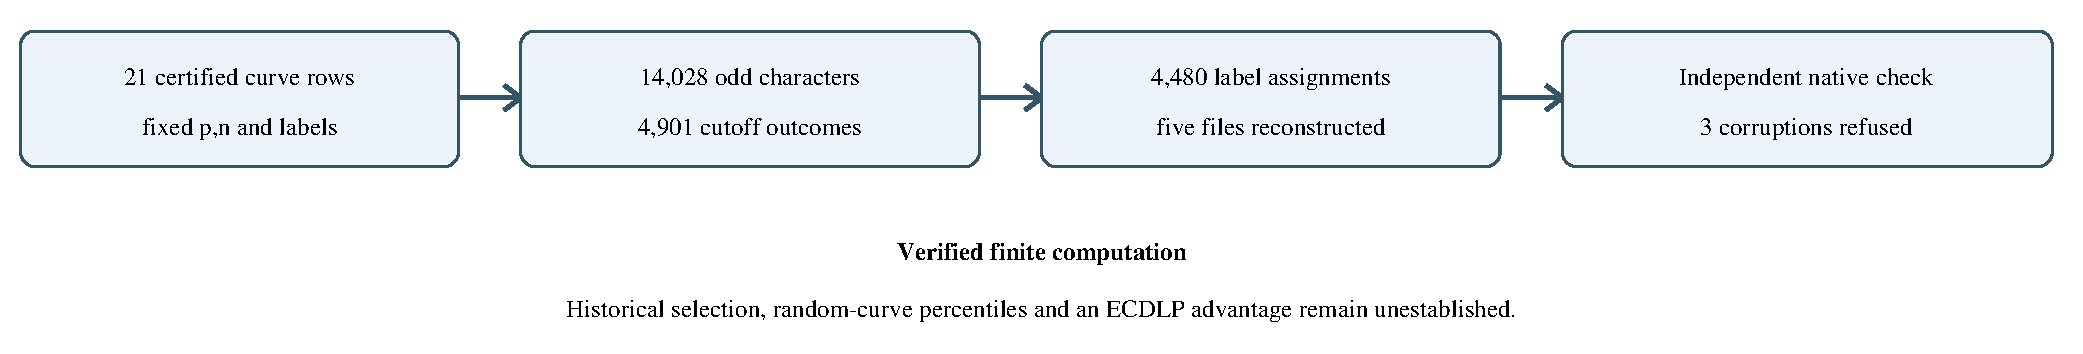
\includegraphics[width=\linewidth]{figures/evidence-boundary.pdf}
\caption{Scope of the independently checked finite calculation.}
\end{figure}
The native GMP producer and separate PARI verifier agree byte-for-byte on five
files, covering 14,028 odd-prime characters, 102,921 curve/cutoff rows, all
4901 cutoff outcomes and all 4480 label assignments. The three altered
character/calibration/summary outputs are each refused with native exit 1.
The implementations may share GMP primitives.

\begin{thebibliography}{9}
\bibitem{asanso} asanso. Prior strict degree-691 observation, 17 October 2026.
\url{https://x.com/asanso/status/2111511837866893580}.
Provenance is the source-bound retrieval recorded in the earlier replication.
\bibitem{replication} Anonymous. \emph{Strict Splitting Counts in Reconstructed
Elliptic-Curve Candidate Streams: An Exact Reproduction and Its Limits}.
Repository draft, 29 October 2026; not submitted. Source paper commit
\texttt{b3e7c31dd70c123d5ba36e5a335c660c40c52d3f}.
\bibitem{ss} I.~E. Shparlinski and A.~V. Sutherland.
\emph{On the Distribution of Atkin and Elkies Primes}.
arXiv:1112.3390v2, 2011.
\bibitem{jmv} D.~Jao, S.~D. Miller and R.~Venkatesan.
\emph{Expander graphs based on GRH with an application to elliptic curve
cryptography}. arXiv:0811.0647v2, 2009.
\end{thebibliography}
\end{document}
